\chapter{Future Work: Deep Hedging Variable Annuities with Transfer Learning} \label{chap:futureWork}

In the evolving landscape of financial markets, insurance products such as VAs have gained a substantial amount of interest due to their ability to provide both investment growth and guaranteed benefits. 
Managing the risks associated with these products, especially in volatile market conditions, is a complex task that demands sophisticated financial modeling techniques. 
Reinforcement Learning (RL) has emerged as a powerful tool for addressing such complexities. With the recent advancement in deep learning, DNN architectures have been successfully applied to RL problems, leading to the development of deep reinforcement learning (DRL) algorithms. 
These algorithms have demonstrated remarkable success decision-making tasks that must be optimized over time. 
In the context of managing VAs, DRL has shown promise in optimizing hedging strategies where long-term financial and policyholder decisions interact dynamically with changing market conditions.

Reinforcement learning is a branch of machine learning in which an agent learns to make sequential decisions by interacting with its environment. 
Through trial and error, the agent receives feedback in the form of rewards or penalties, allowing it to learn an optimal policy for achieving long-term goals. 
In financial and actuarial contexts, RL has been applied to portfolio optimization, asset allocation, and risk management. 
In a dynamic hedging problem, the agent is referred to as the decision-maker that tries to minimize financial risks over time horizon by adjusting the hedging portfolio based on the current environment, which is the current state of the financial markets and actuarial assumptions.
By integrating deep neural network, DRL extends this framework by enabling the agent to handle high-dimensional and complex environments. 
DRL has shown particular promise in finance because of its ability to process vast amounts of financial data and discover intricate patterns in market dynamics.
Despite their success, DRL faces practical limitations when applied to real-world financial markets.
Its most significant drawback is the requirement for extensive data and computational resources.
Training a DRL agent from the scratch requires a large dataset along with considerable computational time for the purpose of exploration and learning.
This is especially problematic for VA contracts, which are long-term insurance products that are sensitive to market fluctuations and underlying actuarial assumptions.
Given that financial markets are highly dynamic, a frequent retraining to account for new market regimes becomes necessary, which can lead to prohibitively high costs and computational inefficiency.
Moreover, using historical data leads to overfitting to the past. 
An overfitting model can lead to suboptimal hedging strategies that perform poorly in changing market conditions.

TL offers a compelling solution to the challenges posed by existing DRL approaches. 
Similar to the TL framework proposed in Chapter~\ref{chap:project3}, TL can also be applied to DRL to accelerate the training.
In the context of financial modeling, instead of training an RL agent from the scratch every time underlying assumptions change, the model can utilize the knowledge gained from past market environments to accelerate the learning process under the new environment.
TL in financial markets is particularly advantageous for addressing the data scarcity problem. 
By transferring existing knowledge from similar environments, TL improves model performance in situations where historical data is limited or noisy. 
This allows models using TL to be both more accurate and computationally efficient. 
Additionally, TL enhances the robustness of models by allowing continuous learning. 
Instead of retraining a deep RL model from the scratch when market conditions shift, TL enables the reuse of pre-trained models, facilitating a faster adaptation to new environments while avoiding overfitting to past conditions.
In the risk management of VA contracts, transfer learning enables quicker adaptation to changing financial and actuarial assumptions by reusing information obtained from another set of related assumptions, such as the management of similar financial instruments or different market regimes. 
A DRL agent equipped with transfer learning can adjust its strategies in response to new market data, making the model more adaptive and responsive without the need for costly retraining.
More specifically, a DRL agent trained to manage VA contracts for a GMMB contract can apply its learned strategies to a GMWB contract with the same financial assumptions. 
A DRL agent trained for a VA product on a Black-Scholes asset model can transfer its knowledge to the training of a similar product on a stochastic volatility model.
This approach substantially reduces the computational costs associated with the training of new VA products with different assumptions and improves the generalization of the model to unseen market conditions.
By integrating the transfer learning with the existing DRL frameworks, we can eliminate the inefficiencies of training models from scratch, provide faster adaptability to new market conditions, and enhance the scalability and computational efficiency of financial models. 
This approach offers a more robust and practical solution for managing VA contracts in dynamic and volatile financial markets.

The rest of the chapter is organized as follows: 
Section~\ref{sec:MDP} introduces the mathematical formulation for hedging VAs and defines the key components of the framework.
Section~\ref{sec:RLAlgorithms} provides an overview of existing RL algorithms and their limitations in the context of hedging VAs.
Section~\ref{sec:PPO} introduces the proximal policy optimization algorithm and its application to the hedging of VAs.
Section~\ref{sec:TL} presents the transfer learning framework for accelerating the training of DRL agents in the dynamic hedging of VAs.
Section~\ref{sec:experiments} presents the experimental setup and results, comparing the performance of transfer learning with training from scratch.
Finally, Section~\ref{sec:FutureDirections} concludes the chapter and discusses future research directions.

\section{Markov Decision Process for Hedging VAs} \label{sec:MDP}

A Markov Decision Process (MDP) provides a mathematical framework for modeling decision-making in stochastic environments over time. 
By formulating the VA hedging problem as an MDP, we can utilize RLalgorithms to learn optimal hedging policies directly from data.
An MDP is defined by the tuple $\mathcal{M} = (\mathcal{S}, \mathcal{A}, \mathcal{P}, \mathcal{R}, \gamma)$, where:

\begin{itemize}
    \item $\mathcal{S}$ is a finite set of states.
    \item $\mathcal{A}$ is a finite set of actions.
    \item $\mathcal{P}$ is a state transition probability distribution, where $\mathcal{P}(s_{t}|s_{t-1}, a_{t-1})$ represents the probability of transitioning from state $s_t$ to state $s_{t-1}$ due to action $a_{t-1}$.
    \item $\mathcal{R}$ is a reward distribution, $\mathcal{R}(s, a, s')$ is the reward received after transitioning from state $s$ to state $s'$ due to action $a$.
    \item $\gamma$ is a discount factor, $\gamma \in [0,1]$,  which models the present value of future rewards.
\end{itemize}

The objective in an MDP is to find a policy, $\pi: \mathcal{S} \rightarrow \mathbb{P}(\mathcal{A})$, that maximizes the cumulative reward over time.
A MDP provides a mathematical framework for solving sequential decision-making tasks in an enviornment where outcomes are partly random and partly under the control of a hedging agent. 
For hedging VAs, the asset dynamics and the mortality model are not controlled by the agent, but the agent controls the cumulative reward by deciding on the hedging weights.
In this section, we reformulate the hedging enviornment of VAs from Section~\ref{subsec:VApayout} as an MDP and define the key components of the MDP.

\subsection{Hedging Environment of Variable Annuities} \label{subsec:VASimulation}

Consider a generic VA contract with maturity $T>0$ periods, e.g., $T=240$ months.
Then the contract expires at $T'=\min\{T,\tau\}$, i.e., the earlier of the contract maturity and the death of the policyholder.
Let $S_t$, $F_t$, and $G_t$ be the indexed stock price, the subaccount value and the guarantee value, respectively, at time $t=1,2,\ldots,T$.
Evolution of the subaccount value and the guarantee value of a VA contract affect the contract payout.
For clarity, we use $F_t$ and $F_{t_+}$ to denote the sub-account value just before and just after the withdrawal at time $t$, if any.
Let $\eta_g$ be the gross rate of management fee that is deducted from the fund value at each period and let $\eta_n < \eta_g$ be the net rate of management fee income to the insurer.
The difference between the gross management fee and the net management fee income represents the incurred investment expenses.

At the inception of the contract, i.e., $t=0$, we assume that the whole premium is invested in the stock index and the guarantee base is set to the sub-account value:
\begin{equation*}
    S_0=F_0=G_0.
\end{equation*}
At each time $t=1,\ldots,T$, the following events take place in the following order:
\begin{enumerate}
    \item The dynamic lapse rate $q_t$ is applied to the contract, i.e., $q$ of the policyholders leave the contract at time $t$.
        \begin{equation} \label{eq3:lapse}
            q_t = q_t^B \cdot \text{clip} (M_q (\frac{G_{t-1}}{F_{t-1}} - D_q), L_q, U_q),
        \end{equation}
    where $q_t^B$ is the base lapse rate, $\text{clip}(x, a, b)$ is a function that clips the value of $x$ to be within the range $[a, b]$, and $M_q$, $D_q$, $L_q$, and $U_q$ are the model parameters taken from National Association of Insurance Commissioners’ (NAIC) Valuation Manual 21~\citep{naic2021}.
    \item The sub-account value changes according to the growth of the underlying stock and the (gross) management fee is deducted. That is, 
        \begin{equation} \label{eq3:subaccount}
            F_t = F_{(t-1)_+}\cdot\frac{S_{t}}{S_{t-1}}\cdot(1-\eta_g)\cdot(1-q_t),
        \end{equation} 
    where $(x)^+=\max\{x,0\}$ and $F_{(t-1)_+}$ will be defined later. The insurer's income at time $t$ is the net management fee, i.e., $F_t\eta_n$. 

    \item The guarantee value ratchets up (ratcheting is a common feature in GMWB) if the sub-account value exceeds the previous guarantee value, i.e., 
        \begin{equation} \label{eq3:guarantee}
            G_t = \max\{G_{t-1}\cdot(1-q_t),F_t\}.
        \end{equation} 
    A GMMB can be modeled with $G_t = G_{t-1}\cdot(1-q_t)$.

    \item The withdrawal is made (for GMWB) and is deducted from the sub-account value, i.e., 
        \begin{equation} \label{eq3:withdrawal}
            F_{t_+} = (F_t - I_t)^+,
        \end{equation} 
    where $I_t = \xi G_t$. A GMMB can be modeled with $\xi = 0$.
\end{enumerate}

Consider a VA contract whose delta hedge portfolio at any time~$t$, $t=0,1,\ldots,T-1$, consists of $\Delta_t$ units in the underlying stock and $B_t$ amount of a risk-free zero-coupon bond maturing at time $T$.
The value of the hedge portfolio at time~$(t-1)$ is:
\begin{equation*}
    H_{t-1} = \Delta_{t-1} S_{t-1} + B_{t-1},
\end{equation*}
where $S_t$ is the underlying stock price and any time $t>0$.
This hedge portfolio is brought forward to the next rebalancing time~$t$, when its value becomes:
\begin{equation*}
    H_{t}^{bf} = \Delta_{t-1} S_{t} + B_{t-1}e^{r}.
\end{equation*}
Therefore, the time~$t$ hedging error, i.e., the cash flow incurred by the insurer due to rebalancing at time~$t$, is
\begin{equation}
    HE_t = H_t - H^{bf}_t, \quad t=1,\ldots, T-1.
\end{equation}
The P\&L of the VA contract includes the cost of the initial hedge ($H_0$), the hedging errors~\eqref{eq2:hedgingerror}, the unwinding of the hedge at maturity ($H^{bf}_T$), and the contract payout at time~$t\in \{0,\ldots,T\}$.
Mathematically, the present value of the liability for a GMMB contract is 
\begin{align} \label{eq3:lossGMMB}
L   & = H_0 - e^{-rT} H^{bf}_T + \sum_{t=1}^{T-1} e^{-rt} HE_t + \sum_{t=1}^T e^{-rt} C_t - \sum_{t=1}^T e^{-rt} F_t\eta_n + e^{-rT} (G_t - F_t)^+  \nonumber \\ 
    & = e^{-rT} (G_T - F_{T^+})^+ + \sum_{t=1}^T e^{-rt}  \left( \Delta_{t-1} (S_{t-1} - e^{-r} S_t) + C_t - F_t\eta_n \right) 
\end{align}
where the equality holds by a rearrangement of terms and a telescopic sum simplification of $e^{-rt}B_t$, $t=0,\ldots,T-1$, and $C_t := C \cdot S_{t-1} \cdot |\Delta_t - \Delta_{t-1}|$ is the tranaction cost at time $t$~\citep{garleanu2013dynamic}.
Hence, the present liability consist of the hedging errors, the transaction costs, the net management fees, and the contract payouts.
Similarly, the present value of the liability for a GMWB contract is
\begin{equation} \label{eq3:lossGMWB}
L = \sum_{t=1}^T e^{-rt}  \left( \Delta_{t-1} (S_{t-1} - e^{-r} S_t) + C_t - F_t\eta_n \right)
\end{equation}
The GMWB payout is implicitly included in $F_t\eta_n$.
Both Equation~\ref{eq3:lossGMMB} and Equation~\ref{eq3:lossGMWB} neglect the transaction cost to liquidate the hedge portfolio at maturity.
The discrete-time hedging problem of VAs can be conveniently formulated as an MDP, where the states, actions, transition probabilities, policies, and rewards are defined as follows.

\subsection{State Space}

The state space $\mathcal{S}$ represents all the information needed to characterize the hedging environment.
In a VA hedging problem, $\mathbf{s}_t$, the information available to a hedging agent at each time $t$ is 
$$\mathbf{s}_t := (S_t, F_t, G_t, \tau, \Delta_{t-1}) \in \mathcal{S}.$$
where $\tau$ is the remaining time to maturity and $\Delta_{t-1}$ is the previous hedging weight.
The hedging environment is partially observed, e.g., the agent does not have access to the contract specifications.
It has to learn a representation of the relevant information from the observed state $\mathbf{s}_t$.

\subsection{Action Space}

The action space $\mathcal{A}$ represents the set of actions that the agent can take at each time $t$.
In a VA hedging problem, the action space only includes the hedging weight $\Delta_t$.

\subsection{Policy}

A policy $\pi$ determines the best action to take in a given state, i.e.,
$$a_t \sim \pi(\cdot|\mathbf{s}_t).$$
In a VA hedging problem the policy outputs the hedging weight $a_t = \Delta_t$ given the observed state $\mathbf{s}_t$.
In the following sections, we will refer to $\Delta_t$ as the policy.

\subsection{Transition Probabilities}

The transition probabilities $\mathcal{P}$ represent the probability of transitioning from one state to another from taking an action.
In our setup, the transition probabilities are fully determined by Equation~\ref{eq3:lapse}, Equation~\ref{eq3:subaccount}, Equation~\ref{eq3:guarantee}, and Equation~\ref{eq3:withdrawal}.
Let $\mathcal{P}(\mathbf{s}_{t+1}|\mathbf{s}_t, a_t)$ be the probability of transitioning from state $\mathbf{s}_t$ to state $\mathbf{s}_{t+1}$ due to action $a_t$.
Aside from the previous hedging weight $\Delta_{t-1}$, the transition probabilities are independent from the actions.
Paths simulated from the transition probabilities are called trajectories (or episodes) of the MDP.

\subsection{Reward and Discount Factor}
The reward function $\mathcal{R}$ and discount factor $\gamma$ in a typical RL problem are defined as follows:
\begin{align}
    \mathcal{R} & = \sum_{t=1}^{T-1} \gamma^t R_t \\
    \gamma      & = e^{-r}, \nonumber
\end{align}
where $R_t$ is the term reward received by the agent at time $t$, and the discount factor $\gamma$ is conveniently inherited from the risk-free rate $r$. 
In hedging, the term reward $R_t$ should be derived from Equation~\ref{eq3:lossGMMB} and Equation~\ref{eq3:lossGMWB} to represent the performance of the hedging policy, i.e., how closely the hedging portfolio tracks the liability.
For the GMWB, we propose a term reward formulation that encourages the agent to maximize the expected reward with low hedging errors and transaction costs:
\begin{equation} \label{eq3:rewardGMWB}
    R_t = F_{t-1}\eta_n - \Delta_{t-1} |S_{t-1} - e^{-r}S_{t}| - C_{t-1}(\Delta_{t-1}), \quad t \in \{1,\ldots,T \}
\end{equation}
The reward function of the GMWB directly links to the time-$t$ loss of a GMWB contract as in Equation~\ref{eq3:lossGMWB}.
The GMMB loss consists of an additional payoff at maturity $T$, thus its term reward is formulated as:
\begin{equation} \label{eq3:rewardGMMB}
    R_t = 
    \begin{cases}
    F_{t-1}\eta_n - \Delta_{t-1} |S_{t-1} - e^{-r}S_{t}| - C_{t-1}(\Delta_{t-1}),                         & t\in \{1,\ldots,T-1 \} \\
    F_{t-1}\eta_n - \Delta_{t-1} |S_{t-1} - e^{-r}S_{t}| - C_{t-1}(\Delta_{t-1}) + (G_T - F_{T^+})^+      & t = T
    \end{cases}
\end{equation}

\subsection{Value Function and Advantage Function}

This section introduces some critical concepts in RL, i.e., the value function and the advantage function.
They are essential for understanding the performance of the hedging policy and the learning process of the RL agent.

A value function quantifies the expected cumulative reward over time.
The state value function, $V^{\pi}(s_t)$, is defined as the expected cumulative reward starting from state $s_t$ and following policy $\pi$ thereafter:

\begin{equation} \label{eq3:V_pi}
    V^{\pi}(s_t) = \mathbb{E} \left[ \sum_{t=0}^{\infty} \gamma^t R_t |\pi, s_t \right],
\end{equation}

where $R_t$ is the reward received by the agent after taking action $a_t$ in state $s_t$ and transitioning to state $s_{t+1}$, and the expectation is taken over the possible sequences of states and rewards that follow from the policy $\pi$.
The state-action value function, $Q^{\pi}(s_t, a_t)$, is defined as the expected cumulative reward starting from state $s_t$, taking action $a_t$, and following policy $\pi$ thereafter:

\begin{equation} \label{eq3:Q_pi}
    Q^{\pi}(s_t, a_t) = \mathbb{E} \left[ \sum_{t=0}^{\infty} \gamma^t R_t |\pi, s_t, a_t \right],
\end{equation}

Based on Equations~\ref{eq3:V_pi} and~\ref{eq3:Q_pi}, the advantage function, $A^{\pi}(s_t, a_t)$, is defined as the difference between the state-action value function and the state value function:

\begin{equation} \label{eq3:A_pi}
    A^{\pi}(s_t, a_t) = Q^{\pi}(s_t, a_t) - V^{\pi}(s_t).
\end{equation}

The advantage function quantifies the advantage of taking action $a_t$ in state $s_t$ over following the policy $\pi$.

\section{Exising RL Algorithms and Their Limitations} \label{sec:RLAlgorithms}

\subsection{Model-Based RL: From AlphaZero to Deep Hedging}
Deep reinforcement learning first attacted attentions when AlphaGo~\citep{silver2016mastering} surpasses human in playing Go. 
Soon after, AlphaZero~\citep{silver2016mastering} emerged as a model-based RL algorithm that improves over self-plays.
It quickly extended beyond Go to other games like Chess and Shogi.
In essence, the AlphaZero agent use a neural network to paramaterize the policy and the value function.
The neural network takes the current state of the game as input and outputs the probability distribution of the next move and a value of the current state.
\begin{equation}
    (\mathbf{\pi}, v) = f_{\theta}(s), \quad L(\theta) = - \mathbf{\pi}^{\intercal} \log(\mathbf{p}) + (z - v)^2  + c||\theta||^2,
\end{equation}
where $f_{\theta}$ is a neural network with parameters $\theta$, $s$ is a current state of the game, $\pi$ is a policy, $v$ is a value of the current state, and $c$ is a regularization parameter.
$\mathbf{p}$ and $z$ are a probability distribution of the next move and an outcome of the game, respectively.
They are induced by a planning algorithm, i.e., Monte Carlo Tree Search (MCTS).
Since it is infeasible to efficiently simulate trajectories in the game of Go, a planning algorithm is necessary to generate expected outcomes.
The neural network $f_{\theta}$ is trained with a stochastic gradient descent algorithm to minimize $L$.
$L$ has three components.
The last term penalizes large neural network weights.
Its first two terms measure the similarity between $f_{\theta}(s)$, the learned policy and value function, with the action and game outcome planned by the MCTS.
The neural network is trained to fit the planned outcomes of the game.
It stores a global solution that predicts the outcome of the game and the next move before they are actually observed.
This is known as model-based RL~\citep{sutton2018reinforcement}.
Using a model allows for planning, i.e., decision-making take place using future situations that have not been experienced by the agent.

In a typical hedging problem, the transition probabilities are independent from the hedging weights, i.e., the actions.
This simplifies the planning as complete trajectories can be simulated without the need of a planning algorithm.
In contrast to AlphaZero, deep hedging~\citep{buehler2019deep} uses monte carlo simulations to generate sample paths of asset dynamics.
These simulations are conducted based on predefined stochastic asset models. 
The parameters and structure of these models are specified in advance, dictating the behavior of the simulated asset prices.

A common choice of $\rho$ is a CVaR.
In practice, the neural network $f_{\theta}$ is trained to minimize the empirical CVaR over a batch of trajectories.
In other words, planning is done through $\rho$, which measures the performance of a hedging policy over a batch of complete trajectories.
The neural network, representing the hedging policy, is trained using the data generated from these simulations. 
The objective is to learn a strategy that minimizes a tail risk measure of the total present liability.
Consequently, the learned policy is inherently tailored to the characteristics of the model used in the simulations.
The ability to know the future outcomes of the hedging policy before they are actually observed and the use of a risk measure to guide the training of the neural network are the key features of model-based RL.
These models describe how asset prices evolve over time, and more importantly, they are used to predict future states based on current information.
While model-based approaches can be powerful when the model accurately reflects reality, they are susceptible to model risk, i.e., the risk that the chosen model is incorrect or incomplete. 
It can lead to suboptimal hedging strategies if the real market deviates from the model assumptions.

For hedging VAs,~\cite{xu2020variable} propose a deep hedging algorithm that falls into this category of model-based RL.
A cost function is defined to minimize the expected shortfall of the total present liability.
~\cite{carbonneau2021deep} extends the model-based approach to hedging long-term financial derivatives and compares the performance of deep hedging strategies trained with different cost functions.
In deep hedging~\citep{buehler2019deep} the state space of the MDP contains the previous hedging weight.
A more recent paper by~\cite{imaki2021no} proposes a new network architecture that removes the previous hedging weight from the state space by introducing a no-transaction band.
It allows for a more efficient training of the neural network by removing the semi-recurrent problem structure.

Despite the success of model-based RL in hedging, most studies focus on hedging different types of contracts on classical asset models, e.g., Black-Scholes model and Heston model.
Motivated by the seminal work by~\cite{gatheral2022volatility}, there are a many subsequent works focusing on roughening the classical stochastic volatility models. 
In the rough volatility models, the latent volatility process is modelled by a stochastic process that is rougher than the sample paths of diffusion process. 
Among these rough volatility models, notable examples are rough Heston model and the rough Bergomi model. 
Model-based RL struggles in a rough volatility model due to difficulties in designing a suitable cost function.~\cite{horvath2021deep} shows that a standard implementation of deep hedging can lead to suboptimal hedging performance in a discretized rough Bergomi model. 

In contrast, a model-free approach does not require a explicit design for different asset dynamics, making it more flexible and adaptable to different market conditions and more robust to model misspecification.

\subsection{Model-Free RL for Hedging}
    
In a model-free reinforcement learning approach, the agent is a trial-and-error learner that interacts with the environment to learn the optimal policy by iteratively updating the policy and the value function based on the observed states, actions, and rewards.
For hedging VAs, the agent does not have access to a planning algorithm or the underlying stochastic asset model, and it must learn the optimal policy by directly interacting with the environment.

Model-free RL algorithms gain its popularity in robotics tasks, where transition probabilities in the environment are unknown and can be affected by the agent's actions.
In the context of hedging, existing studies use transaction costs as a function of the hedging weights, which makes the transition probabilities independent on the actions.
However, the trade size can affect the asset price in a real environment~\citep{hasbrouck1991measuring}, which makes the model-free approach a promising direction for hedging VAs in the real market.

Boardly speaking, model-free RL can be categorized into two types: value-based RL and policy-based RL.
Value-based approaches learn the value function directly from the data and derive the policy from the learned value function. 
The value function is learned by training a DNN to approximate the value function, which quantifies the expected cumulative reward over time. 
The policy is then derived from the learned value function by selecting the action that maximizes the value function at each state. 
~\cite{mnih2015human} is the first paper to demonstrate the effectiveness of value-based deep reinforcement learning in training agents to play Atari games.
To update the value function, the DNN is trained to minimize the difference between the current value function and the target value function, which is updated based on the maximum expected reward from the previous iteration.
When trained to approximate the value function, the DNN benefits from the use of experience replay buffers, which is proposed by~\cite{lin1992self} to store and sample historical transitions and uniformly sampled during training to enhance the sample efficiency and stability of the learning process.
~\cite{kolm2019dynamic} uses a value-based deep reinforcement learning approach to hedge European options under the Black-Scholes framework.

In valued-based approaches, the value function is updated iteratively with the maximum expected reward of all possible actions, which can be computationally expensive for continuous action spaces.
To overcome this difficulty, a policy-based approach estimates the value function before realization of the final payoff of the hedging portfolio, which is particularly useful for hedging long-term financial derivatives or VA contracts.
Two types of policy-based approaches prevail in the literature: actor-critic and policy gradient methods.

An actor-critic method designs an actor network and a critic network to learn the value function and the policy simultaneously.
The actor network learns the policy by directly outputting the action based on the current state, while the critic network learns the value of an action by approximating the expected cumulative reward over time following the actor's policy.
A popular actor-critic algorithm is the Deep Deterministic Policy Gradient (DDPG) algorithm proposed by~\cite{lillicrap2015continuous}, which is implemented by~\cite{xu2022delta} in hedging financial derivatives in S\&P 500 and DJIA index options.

A policy gradient method uses policy gradient theorem to update the policy by performing gradient ascent with respect to the policy parameters.

\begin{algorithm}[H] 
    \caption{Vanilla Policy Gradient (REINFORCE)}
    \begin{algorithmic}[1] \label{alg:REINFORCE}
    \STATE \textbf{Initialize} policy parameters $\theta$ arbitrarily.
    \STATE  \textbf{For} {iteration $k=0, 1,2,\ldots$} \textbf{do}
        \STATE \quad  Collect a set of $\mathcal{D}_k$ by sampling from the enviornment with policy $\pi_\theta$.
        \STATE  \quad Compute the rewards $R_t$ for each trajectory in $\mathcal{D}_k$ for $t=0,1,\ldots,T$.
        \STATE  \quad Update the policy parameters $\theta_{k+1}$ by 
        \begin{equation*}
            \theta_{k+1} = \theta_k + \alpha \frac{1}{|\mathcal{D}_k|T} \sum_{\mathcal{\kappa} \in \mathcal{D}_k} \sum_{t=0}^{T} \nabla_\theta \log \pi_\theta(a_t | s_t) R_t
        \end{equation*}
    \STATE  \textbf{End For}
    \end{algorithmic}
\end{algorithm}

Algorithm~\ref{alg:REINFORCE} shows the REINFORCE algorithm~\citep{sutton1999policy}, a classic policy gradient method that updates the policy by performing gradient ascent with respect to the policy parameters.
When training on real-world data, deep hedging of~\cite{buehler2019deep} effectively becomes a model-free policy gradient methods. 
The policy is updated by performing gradient ascent with respect to the policy parameters to maximize the expected reward over time, where the reward function is designed to be the negative of a tail risk measure of the total present liability.

Representative algorithms include the Trust Region Policy Optimization (TRPO) algorithm proposed by~\cite{schulman2015trust} and the Proximal Policy Optimization (PPO) algorithm proposed by~\cite{schulman2017proximal}.
~\cite{du2020deep} show that the PPO algorithm is more sample efficient and stable than the value-based approaches in training agents to hedge financial derivatives.
The most relevant paper to our study is~\cite{chong2023pseudo}, which uses the PPO algorithm to hedge GMMB with a GMDB rider under the Black-Scholes framework.
However, information of the underlying risk factors is leaked to the agent, which makes their study pseudo-model-free.
To further improve the risk management of VAs under rough volatility models, we propose a model-free deep reinforcement learning approach to hedge VAs without explicit or implicit knowledge of the underlying risk factors.

\section{Hedging VAs with a PPO Agent} \label{sec:PPO}
In a hedging problem, an insurer aims at finding a policy $\pi$ that maximizes the expected reward over time.
In a policy-based RL approach like the PPO, both the policy and the value function are parameterized by deep neural networks.
We denote the policy by $\pi_{\theta}$ and the value function by $V_{\phi}$, where $\theta$ and $\phi$ are the parameters of the value network and the policy network, respectively.
The policy is updated according to an objective function that reflects the advantage of taking action $a_t$ in state $s_t$ over following the policy $\pi$.
\begin{align}
    \max_{\theta} \mathbb{E}\left[ \min \left\{ \Lambda_t(\theta)\hat{A}^{\pi_{\theta}}(s_t, a_t), \text{clip}(\Lambda_t(\theta), 1-\epsilon, 1 + \epsilon) \hat{A}^{\pi_{\theta}}(s_t, a_t)  \right\} \right] \\
    \Lambda_t(\theta) = \frac{\pi_{\theta}(a_t|s_t)}{\pi_{\theta_{old}}(a_t|s_t)} 
\end{align}
where $\theta_{old}$ denotes the policy parameters at the previous iteration, $\epsilon$ is a clip range hyperparameter that controls the size of the policy update, $\text{clip}(x, a, b)$ is a function that clips the value of $x$ to be within the range $[a, b]$, and $\hat{A}^{\pi_{\theta}}(s_t, a_t)$ is an estimated advantage of taking action $a_t$ in state $s_t$ over following the policy $\pi_{\theta_{old}}$.
In our implementation, the advantage function is estimated following the GAE method proposed by~\cite{schulman2015high}.
The policy is updated by performing gradient ascent with respect to the policy parameters $\theta$ to maximize the objective function, which is estimated by sampling from the environment and computing the empirical average of the objective function over the sampled trajectories.
The first component in the objective function, $\Lambda_t(\theta) \hat{A}^{\pi_{\theta}}(s_t, a_t)$, is a surrogate objective function that approximates the advantage of taking action $a_t$ in state $s_t$ over following the policy $\pi_{\theta_{old}}$, and the second component, $\text{clip}(\Lambda_t(\theta), 1-\epsilon, 1 + \epsilon) \hat{A}^{\pi_{\theta}}(s_t, a_t)$, is a clipped surrogate objective function that prevents large policy updates and ensures more stable training.
The TRPO algorithm proposed by~\cite{schulman2015trust} uses a similar clipped surrogate objective function to ensure that the policy update does not deviate too far from the old policy, but PPO simplifies the optimization problem by using a clipped surrogate objective function instead of a hard-coded constraint on the policy update.
Compared to TRPO, PPO is more computationally efficient and easier to implement, making it a popular choice for training deep reinforcement learning agents.
For a in-depth discussion on the implementation details of both TRPO and PPO, we refer the reader to~\cite{engstrom2020implementation}.

\begin{algorithm} 
    \caption{PPO for Hedging Variable Annuities} 
    \begin{algorithmic}[1] \label{alg3:ppoHedging}
        \STATE  Initialize policy parameters $\theta_0$ and value function parameters $\phi_0$.
        \STATE  \textbf{For} {iteration $k=0, 1,2,\ldots$} \textbf{do}
        \STATE  \quad Collect a set of trajectories $\mathcal{D}_k$ by sampling from the environment with policy $\pi_{\theta_{k}}$.
        \STATE  \quad Compute the rewards $\hat{R}_t$ for each trajectory in $\mathcal{D}_k$.
        \STATE  \quad Estimates the advantage function with $\hat{A}_{\pi_{\theta_k}}(\mathbf{s}_t, a_t)$ using value function $V_{\phi_k}$.
        \STATE  \quad Update the policy parameters $\theta_{k+1}$ by 
        \begin{equation*}
            \max_{\theta} \mathbb{E}\left[ \min \left\{ \Lambda_t(\theta)\hat{A}^{\pi_{\theta}}(\mathbf{s}_t, a_t), \text{clip}(\Lambda_t(\theta), 1-\epsilon, 1 + \epsilon) \hat{A}^{\pi_{\theta}}(\mathbf{s}_t, a_t)  \right\} \right]
        \end{equation*}
        \STATE  \quad Update the value function parameters $\phi_{k+1}$ by minimizing the mean squared error between the predicted value and the actual collected reward.
        \begin{equation*}
            \phi_{k+1} = \arg \min_{\phi} \frac{1}{|\mathcal{D}_k|T} \sum_{\mathcal{\kappa} \in \mathcal{D}_k} \sum_{t=0}^{T} \left( V_{\phi}(\mathbf{s}_t) - \hat{R}_t \right)^2
        \end{equation*}
        \STATE  \textbf{End For}
    \end{algorithmic}
\end{algorithm}

Algorithm~\ref{alg3:ppoHedging} outlines the PPO algorithm for training an agent to hedge VAs.
At each iteration $k$, the agent collects a set of trajectories $\mathcal{D}_k$ by interacting with the environment (Section~\ref{subsec:VASimulation}) with the current policy $\pi_{\theta_k}$.
The agent then computes the rewards $\hat{R}_t$ for each trajectory in $\mathcal{D}_k$ and estimates the advantage function with $\hat{A}_{\pi_{\theta_k}}(s_t, a_t)$ using the value function $V_{\phi_k}$.
The policy parameters $\theta_{k+1}$ are updated by performing gradient ascent with respect to the policy parameters to maximize the clipped surrogate objective function.
The value function parameters $\phi_{k+1}$ are updated by minimizing the mean squared error between the predicted value and the actual collected reward.
The agent iterates this process until convergence to learn an optimal policy for hedging VAs.

\subsection{Accounting for Non-Markovian Dynamics}

In the context of hedging VAs, the state space is partially observed.
The agent does not have access to the contract specifications and the underlying risk factors.
Furthermore, a rough volatility model introduces non-Markovian dynamics, i.e., the future state of the system depends on the entire history of the system.
To address the non-Markovian dynamics, an LSTM component is added to the state representation $\mathbf{s}_t$ to capture the temporal dependencies in the data.
This approach is known as recurrent PPO~\citep{ni2021recurrent}.
Let $h_t$ be the hidden state of the LSTM at time $t$.
The state representation $\mathbf{s}_t$ is fed into the LSTM at each time step to update the hidden state $h_t$.
\begin{equation} \label{eq3:stateRNN}
    \mathbf{s}_t = (S_t, F_t, G_t, \tau, \Delta_{t-1}), \quad h_t = \text{LSTM}(\mathbf{s}_t, h_{t-1})
\end{equation}

In a LSTM, the cell state $c_t$ stores a representation of historical information up to time $t$.
It is updated at each time step by a forget gate $f_t$, an input gate $i_t$, and an output gate $o_t$.

In a recurrent PPO with LSTM, the policy and reward function remain the same but with the new state representation in Equation~\ref{eq3:stateRNN}.
Instead of following the standard PPO algorithm, the agent uses the recurrent PPO algorithm to learn an optimal policy for hedging VAs.
Figure~\ref{fig3:architecturePPO} illustrates the network architecture of the standard PPO and the recurrent PPO with LSTM, and Algorithm~\ref{alg3:ppoHedging-rnn} outlines the recurrent PPO algorithm and for training an agent to hedge VAs with non-Markovian dynamics.

\begin{algorithm}
    \caption{Recurrent PPO with LSTM for Hedging Variable Annuities} 
    \begin{algorithmic}[1] \label{alg3:ppoHedging-rnn}
        \STATE  Initialize policy parameters $\theta_0$ and value function parameters $\phi_0$.
        \STATE  Initialize the LSTM layers with random weights, and set the hidden state $h_0$ to zeros.
        \STATE  \textbf{For} {iteration $k=0, 1,2,\ldots$} \textbf{do}
        \STATE  \quad Collect a set of trajectories $\mathcal{D}_k$ by sampling from the environment with policy $\pi_{\theta_{k}}$.
        \STATE  \quad Reset the LSTM hidden state $h_0$ to zeros at the beginning of each trajectory.
        \STATE  \quad Compute the rewards $\hat{R}_t$ for each trajectory in $\mathcal{D}_k$.
        \STATE  \quad Estimates the advantage function with $\hat{A}_{\pi_{\theta_k}}(\mathbf{s}_t, a_t)$ using value function $V_{\phi_k}$.
        \STATE  \quad Update the policy parameters $\theta_{k+1}$ by 
        \begin{equation*}
            \max_{\theta} \mathbb{E}\left[ \min \left\{ \Lambda_t(\theta)\hat{A}^{\pi_{\theta}}(\mathbf{s}_t, a_t), \text{clip}(\Lambda_t(\theta), 1-\epsilon, 1 + \epsilon) \hat{A}^{\pi_{\theta}}(\mathbf{s}_t, a_t)  \right\} \right]
        \end{equation*}
        \STATE  \quad Update the value function parameters $\phi_{k+1}$ by minimizing the mean squared error between the predicted value and the actual collected reward.
        \begin{equation*}
            \phi_{k+1} = \arg \min_{\phi} \frac{1}{|\mathcal{D}_k|T} \sum_{\mathcal{\kappa} \in \mathcal{D}_k} \sum_{t=0}^{T} \left( V_{\phi}(\mathbf{s}_t) - \hat{R}_t \right)^2
        \end{equation*}
        \STATE  \textbf{End For}
    \end{algorithmic}
\end{algorithm}

\begin{figure}[ht!]
    \centering
    \begin{subfigure}{0.45\textwidth}
        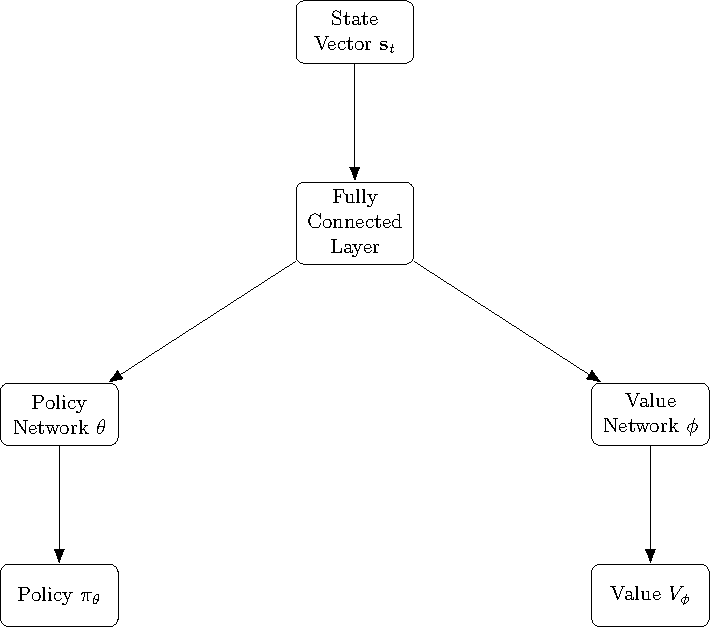
\includegraphics[width=\textwidth]{./futureWork/tikz/ppo_diagram.pdf}
        \caption{regular PPO}
        \label{subfig3:architecturePPO}
    \end{subfigure}
    \hspace{1cm}
    \begin{subfigure}{0.45\textwidth}
        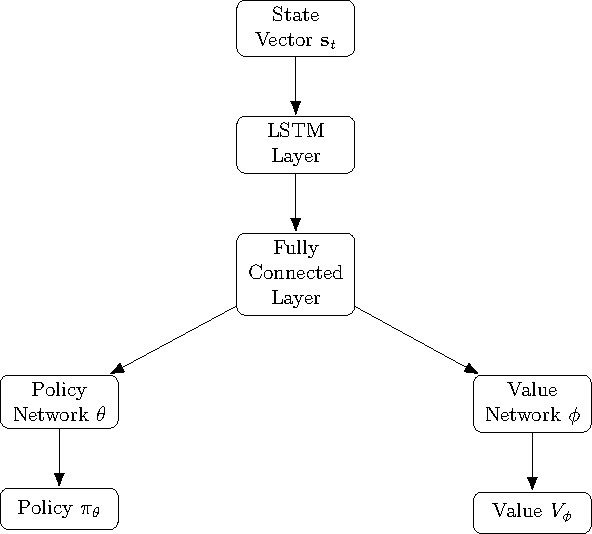
\includegraphics[width=\textwidth]{./futureWork/tikz/recurrentppo_diagram.pdf}
        \caption{Recurrent PPO with LSTM}
        \label{subfig3:architectureLSTMPPO}
    \end{subfigure}
    \caption{PPO Network Architectures} 
    \label{fig3:architecturePPO}
\end{figure}

The recurrent PPO algorithm is similar to the standard PPO algorithm, but it includes an LSTM component to capture the temporal dependencies in the data.
However, the sequantial nature of the LSTM is not suitable for a parallel computation, which slows down the training process.

\section{Transfer Learning for Hedging VAs} \label{sec:TransferLearning}

In the context of deep hedging, various research has been conducted to improve the hedging strategies on real-world data by leveraging knowledge from simulated data.
Most of the research uses the offline-online learning approach, where the hedging strategies are first trained with simulation data, but updated in real-time based on new market information and continuous learning to adapt to changing market dynamics.
The most relevant paper to our study is~\cite{xiao2021optimal}, which use policy gradient algorithms to train hedging strategies for European options with simulation data from Heston model and then updated in real-time hedging S\&P 500 index options.
To the best of our knowledge, no research has been conducted to improve the hedging strategies with the state-of-the-art transfer learning techniques.
This section introduces some transfer learning techniques that are relevant to our task of hedging VAs.

\subsection{Reward Shaping}

In the context of hedging VAs using deep reinforcement learning and transfer learning, reward shaping becomes a crucial technique. 
It involves modifying the reward function in the target domain to incorporate additional guidance, which often leads to more efficient learning and a better performance.
This technique can be particularly useful for managing the complex risks associated with VAs, as it can guide the learning process towards strategies that are more effective in hedging these products.

One way to implement reward shaping in this context is by introducing auxiliary rewards that reflect the performance of hedging strategies learned from the source domains.
Reward shaping learns an auxiliary reward function $\mathcal{R}_s: \mathcal{S} \times \mathcal{A} \times \mathcal{S} \rightarrow \mathbb{R}$ from the source domains.
The auxiliary reward function is then used to shape the reward function in the target domain, $\mathcal{R}'_t = \mathcal{R}_t + \mathcal{R}_s$, by incorporating the insights gained from the source domains.

Some popular reward shaping techniques include potential-based reward shaping~\citep{ng1999policy}, potential-based state-action advice~\citep{wiewiora2003principled}, dynamic value function advice~\citep{harutyunyan2015expressing}.

\subsection{Policy Transfer}

The most straightforward approach to transfer learning is to directly transfer the policy learned from the source domains to the target domain via policy distillation.
Policy distillation is a technique that transfers the knowledge from a teacher policy to a student policy by training the student policy to mimic the teacher policy up to a certain extent.
The teacher policy is learned from the source domains, and the student policy learns the hedging strategies in the target domain while guided by the teacher policy.
In the Distral algorithm~\citep{teh2017distral}, the student policy maximizes a multi-task objective:
$\max_{\phi} \sum_{i=1}^K \mathcal{J}(\pi_\phi, \pi_{E_i})$, where

\begin{equation}
    \mathcal{J}(\pi_\phi, \pi_{E_i}) = \sum_{t=0}^\infty \mathbb{E}_{s_t \sim \mu_0^t, a_t \sim \pi_\phi} \left[ \gamma^t R_{t+1} + \frac{\alpha}{\beta} \log \pi_{\phi}(a_t|s_t) - \frac{1}{\beta}log \pi_{E_i}(a_t|s_t) \right],
\end{equation}

where a set of $K$ teacher policies $\pi_{E_i}$ are learned from the source domains, and the student policy $\pi_\phi$ is learned on the target domain. $\alpha$ and $\beta$ are hyperparameters that control the trade-off between mimicking the teacher policies and exploring the target domain.

\subsection{Evaluation Metrics}

The metrics discussed for evaluating transfer learning approaches focus on two key aspects: mastery and generalization. 
Mastery assesses the agent's final performance level in the target domain, indicating how effectively it has learned a specific task from previous knowledge. 
Some common metrics for evaluating mastery include:
Generalization, on the other hand, refers to the agent's ability to quickly adapt its learned knowledge to the target domain.
In the context of risk management, generalization is more important than mastery, as the agent must be able to quickly adapt to changing market conditions and new financial products.
Some common metrics for evaluating generalization include:

\begin{itemize}
    \item \textbf{Jumpstart performance:} the initial reward of the agent in the target domain.
    \item \textbf{Accumulated reward:} the total area under the reward curve over time in the target domain.
    \item \textbf{Time to threshold:} the time it takes for the agent to reach a certain performance threshold in the target domain.
    \item \textbf{Performance with fixed epochs:} the agent's performance in the target domain after a fixed number of epochs.
\end{itemize}

\section{Numerical Experiments} \label{sec:Experiments}

We present a numerical experiment to demonstrate the effectiveness of the model-free PPO algorithm for hedging VAs with transaction costs.
We consider a VA contract with a maturity of $T=240$ months and a GMMB rider with a simulation environment described in Section~\ref{subsec:VASimulation}.
The simulation enviornment is implemented in Python using the OpenAI Gym framework~\citep{brockman2016openai}, and the neural networks are programmed using the PyTorch library~\citep{paszke2019pytorch}.
The environment is designed to simulate the dynamics of the VA contract and provide the agent with the current state of the VA with the contract specifications and the financial market information described in Table~\ref{tab3:hyperparameters}.

\begin{table}[ht!]
    \centering
    \begin{tabular}{ll} 
        \toprule
        Hyperparameter      & Value \\
        \midrule
        $|\mathcal{D}_k|$   & 16        \\
        $\epsilon$          & 0.2       \\
        Learning rate       & 0.0001    \\
        $S_0$               & 1000      \\
        $\mu$               & 0.00375   \\
        $\sigma$            & 0.0457627 \\
        $r$                 & 0.002     \\
        $T$                 & 240       \\
        \bottomrule
    \end{tabular}
    \caption{PPO Hyperparameters and GMMB Contract Specifications} 
    \label{tab3:hyperparameters}
\end{table}

The underlying asset price $S_t$ is modeled as a geometric Brownian motion (GBM) with a drift rate $\mu$ and a volatility $\sigma$.

\begin{figure}
    \centering
    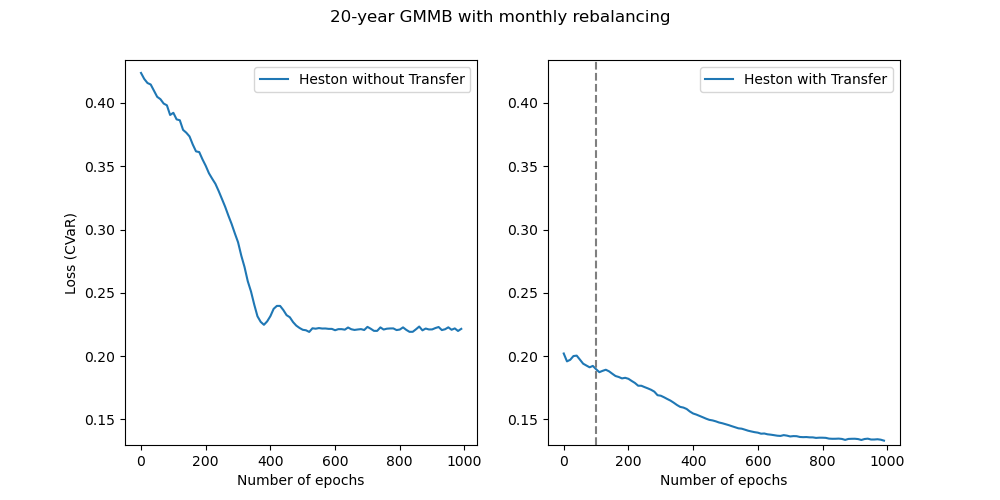
\includegraphics[width=0.9\textwidth]{./futureWork/figures/CVaR_histories.png}
    \caption{Hedging performance of deep hedging with transfer learning}
    \label{fig3:dh-transfers}
\end{figure}

Figure~\ref{fig3:dh-transfers} illustrates the hedging performance of the deep hedging algorithm with transfer learning for hedging VAs with a GMMB rider.
The first deep hedging agent is directly trained on the Heston asset model, and the second deep hedging agent is trained with transfer learning from the GBM model.
The figure plot the 95\%-CVaR of hedging errors against training epochs for both agents.
The deep hedging agent with transfer learning outperforms the deep hedging agent trained on the Heston model in both mastery and generalization.
The agent with transfer learning achieves a lower loss in the target domain and adapts more quickly to the new environment, indicating that the agent has learned a more robust hedging strategy that can be effectively applied to a more complex environment.

For the PPO agent, we use a regular PPO and a recurrent PPO with an LSTM component to capture the temporal dependencies in the data.
The weights of the value network and the policy network are initialized with orthogonal initialization~\citep{engstrom2020implementation} with scaling $\sqrt{2}$ and the bias terms set to zero.
The value network and the policy network are implemented as fully connected neural networks with two hidden layers of 16 units each and $\tanh$ activation functions.
They are trained using the Adam optimizer with a learning rate of $0.0001$ and a batch size automatically adjusted to the number of trajectories in the collected dataset.
At each timestep, the observations are normalized and cliped between $-10$ and $10$ before being fed into the neural networks to stabilize the training process.
For PPO, we follow the suggestions in~\cite{schulman2017proximal} and set the clipping hyperparameter $\epsilon$ to $0.2$ to prevent large policy updates. 
More specifically, our implementation of the PPO uses a generalized advantage estimation~\citep{schulman2015high} to estimate the advantage function.
The agent interacts with the environment for $10^5$ episodes, and the policy and value networks are evaluated every $1000$ episodes.
The performance of the agent is evaluated based on the average reward over an independent test set of $10^3$ episodes, and the results are compared with the benchmark hedging strategy, delta hedging.

\begin{figure}[ht!]
    \centering
    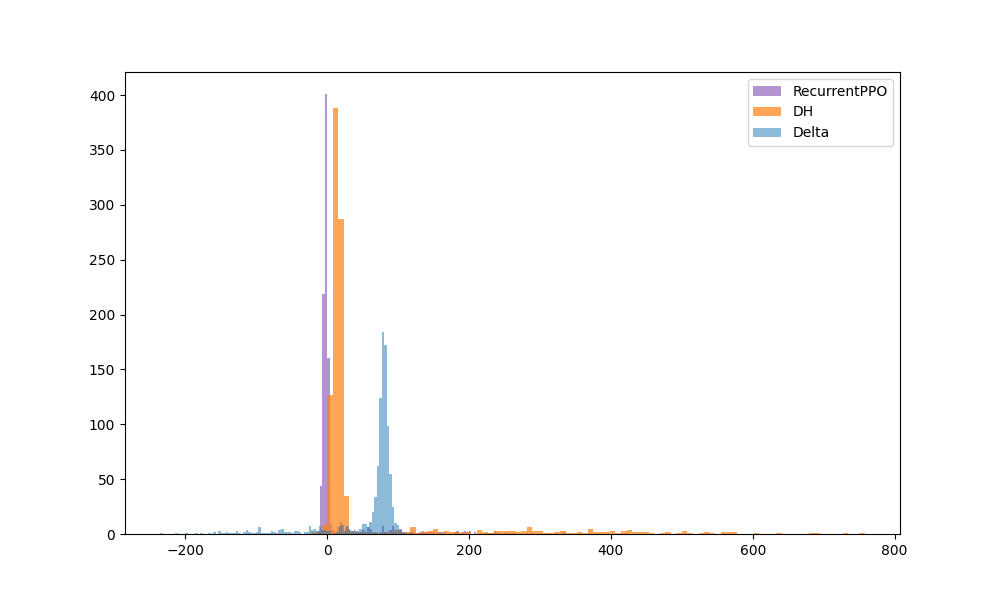
\includegraphics[width=0.5\textwidth]{./futureWork/figures/PPO_DH.png}
    \caption{Hedging performance of recurrent PPO and deep hedging}
    \label{fig3:ppo_dh}
\end{figure}

This experiment compares the hedging performance of the recurrent PPO agent with LSTM and the deep hedging algorithm proposed by~\cite{buehler2019deep} for hedging VAs with a GMMB rider.
The experiment is conducted with the same amount ofsimulation budget.

\begin{figure}[ht!]
    \centering
    \begin{subfigure}{0.45\textwidth}
        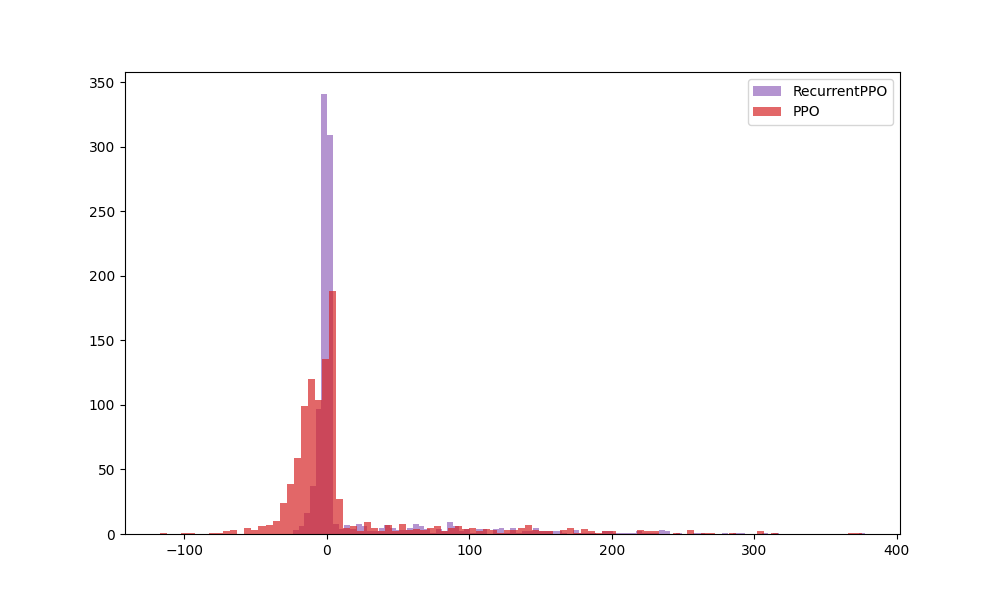
\includegraphics[width=\textwidth]{./futureWork/figures/PPOs_GBM.png}
        \caption{GBM}
    \end{subfigure}
    \hspace{1cm}
    \begin{subfigure}{0.45\textwidth}
        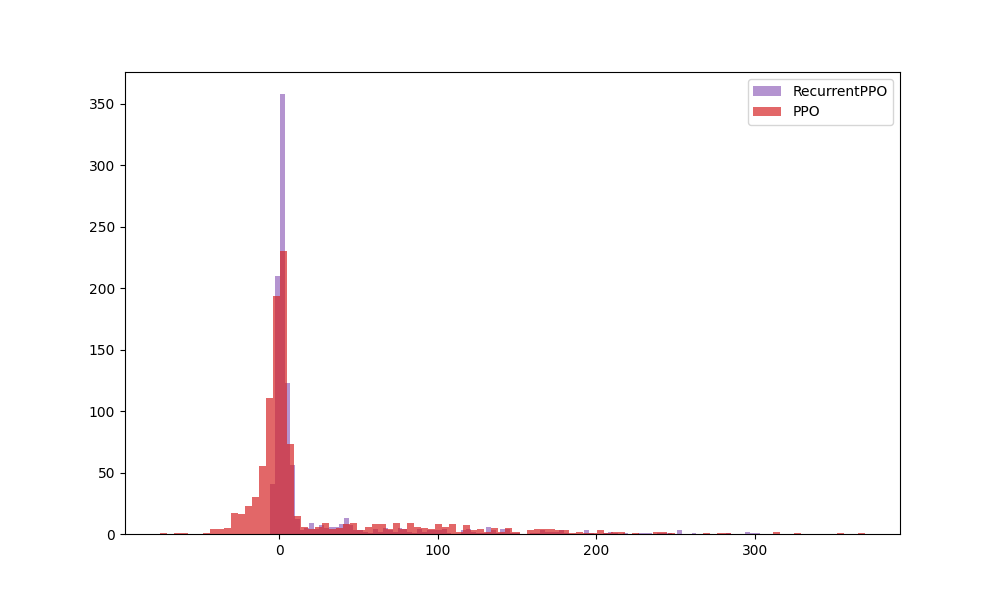
\includegraphics[width=\textwidth]{./futureWork/figures/PPOs_GBMRS.png}
        \caption{Regime-switching GBM}
    \end{subfigure}
    \caption{Hedging performance of standard PPO and recurrent PPO} 
    \label{fig3:ppo_result}
\end{figure}

Figure~\ref{fig3:ppo_result} illustrates the hedging performance of the standard PPO and the recurrent PPO with LSTM for hedging VAs with transaction costs $C=0.005$.
The figures show the distributions of the hedging errors incurred by the agents over the $10^3$ test episodes for the GBM and the regime-switching GBM asset models.
For both asset models, the recurrent PPO outperforms the standard PPO in terms of hedging performance.
For the regime-switching GBM, the 95\%-VaR of hedging errors of the recurrent PPO and the standard PPO are $136.24$ and $147.14$, respectively.
The hedging errors of the recurrent PPO are more concentrated around zero, indicating that historical information captured by the LSTM component helps the agent make better hedging decisions even in the enviornment is Markovian.

\begin{figure}[ht!]
    \centering
    \begin{subfigure}{0.45\textwidth}
        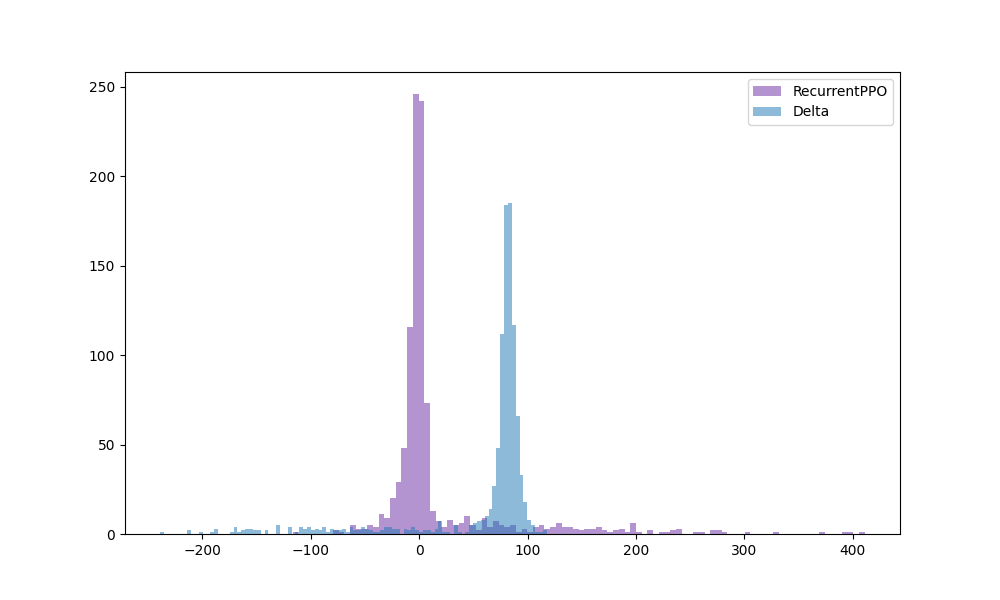
\includegraphics[width=\textwidth]{./futureWork/figures/PPO_cost_001.png}
        \caption{$C = 0.001$}
    \end{subfigure}
    \hspace{1cm}
    \begin{subfigure}{0.45\textwidth}
        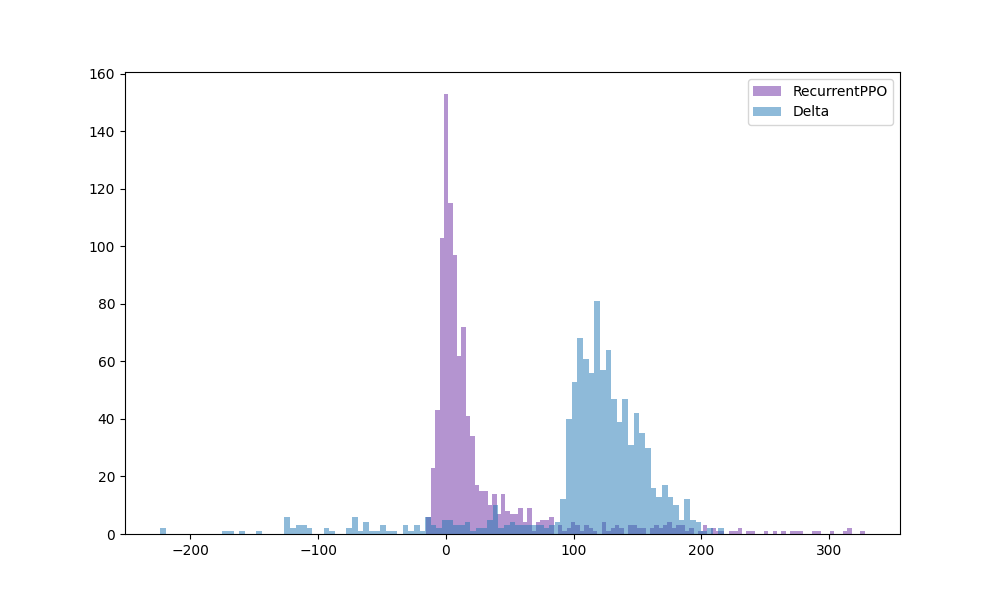
\includegraphics[width=\textwidth]{./futureWork/figures/PPO_cost_02.png}
        \caption{$C = 0.02$}
    \end{subfigure}
    \caption{Hedging performance of recurrent PPO and delta hedging with different transaction costs} 
    \label{fig3:ppo_cost}
\end{figure}

Figure~\ref{fig3:ppo_cost} shows the hedging performance of the recurrent PPO agent and the delta hedging strategy with different transaction costs when the asset model is a GBM.
The experiment is conducted with transaction costs of $C=0.001$ and $C=0.02$.
The delta hedging strategy is implemented with the Black-Scholes delta.
When the transaction cost is low, the delta hedging strategy outperforms the recurrent PPO agent.
However, as the transaction cost increases, delta hedging becomes less effective, and the recurrent PPO agent is able to learn from the environment and adapt its hedging strategy to minimize the hedging errors.

\begin{figure}[ht!]
    \centering
    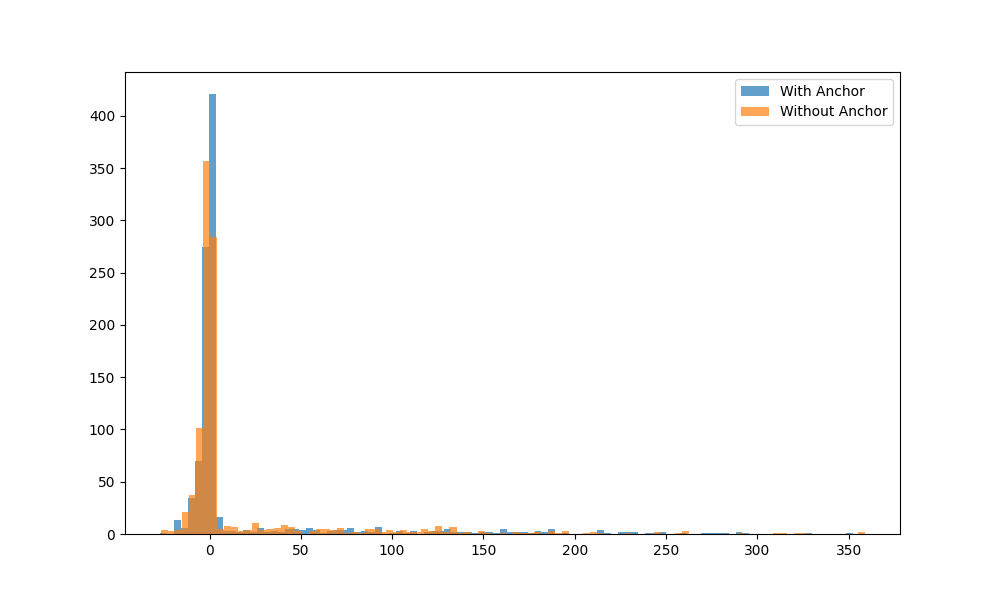
\includegraphics[width=\textwidth]{./futureWork/figures/PPO_anchor.png}
    \caption{Hedging performance of recurrent PPO with or without anchor}
    \label{fig3:ppo_anchor}
\end{figure}

Figure~\ref{fig3:ppo_anchor} illustrates the hedging performance of the recurrent PPO agent with and without the model information of the underlying asset model and the current value of the liability.
The experiment is conducted for the GBM asset model with transaction costs of $C=0.005$.
The results show that the agent with the model information does not outperform the agent without the model information.


\begin{figure}[ht!]
    \centering
    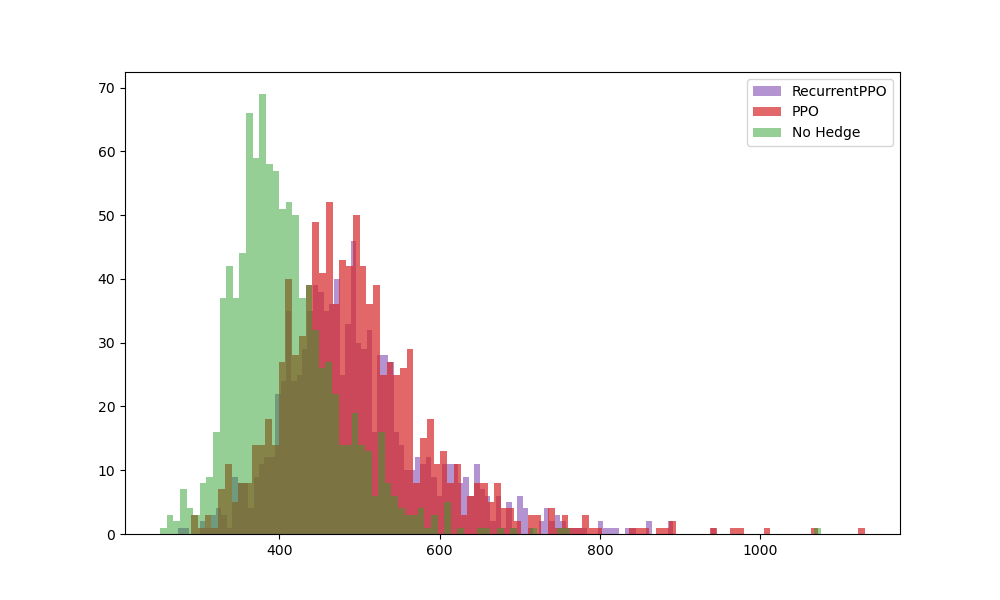
\includegraphics[width=\textwidth]{./futureWork/figures/PPO_GMWB.png}
    \caption{Hedging performance of recurrent PPO with GMWB}
    \label{fig3:ppo_GMWB}
\end{figure}

Figure~\ref{fig3:ppo_GMWB} illustrates the hedging performance of the recurrent PPO agent for hedging VAs with a GMWB rider.
The experiment is conducted with the same hyperparameters as the experiment with the GMMB rider.
Unlike the GMMB rider, the PPO agent struggles to learn an optimal hedging strategy for the VA with a GMWB rider.
The hedging errors of the PPO agent are more dispersed, indicating that more training episodes are needed to achieve a satisfactory hedging performance.
The results suggest that the GMWB rider introduces additional complexity to the hedging problem, and the model-free RL algorithm is not sample efficient.

\section{Future Directions} \label{sec:FutureDirections}

The proposed future work of this thesis aims at investigating how transfer learning can be effectively integrated into the training of PPO agents for dynamic hedging of VA contracts. 
The primary goal is to enhance the adaptability and efficiency of hedging strategies in response to new VA products and changing market conditions. 


The first objective is to establish a systematic approach for transferring policies learned by PPO agents from source tasks to target tasks in the context of dynamic hedging. 
Source tasks may involve hedging a GMMB under a specific market model, while target tasks could entail hedging a GMWB under a different market model.

To achieve this, the research will explore methodologies such as policy distillation, where knowledge from a pre-trained "teacher" policy is transferred to a "student" policy~\citep{rusu2015policy}.
Policy distillation has been effective in compressing and transferring knowledge between networks, improving learning efficiency in RL settings.
Another avenue for future research is the use of pre-trained model initialization, wherein the policy network trained on the source task initializes the policy for the target task. 
This method leverages the shared underlying structures between tasks, which can potentially accelerate convergence and improve performance.
The framework will also consider feature representation transfer, which aims at reusing learned representations of market dynamics and policyholder behaviors between tasks. 
By capturing common patterns across different contracts and market models, the PPO agent can more effectively generalize to new scenarios~\citep{bengio2012deep}.

By addressing these objectives, the research aims at advancing the field of financial risk management through the development of adaptive and efficient hedging strategies for VA contracts. The integration of transfer learning into PPO agents has the potential to substantially reduce computational costs and improve the robustness of hedging policies in dynamic market environments.